% Options for packages loaded elsewhere
\PassOptionsToPackage{unicode}{hyperref}
\PassOptionsToPackage{hyphens}{url}
%
\documentclass[
]{article}
\usepackage{amsmath,amssymb}
\usepackage{lmodern}
\usepackage{iftex}
\ifPDFTeX
  \usepackage[T1]{fontenc}
  \usepackage[utf8]{inputenc}
  \usepackage{textcomp} % provide euro and other symbols
\else % if luatex or xetex
  \usepackage{unicode-math}
  \defaultfontfeatures{Scale=MatchLowercase}
  \defaultfontfeatures[\rmfamily]{Ligatures=TeX,Scale=1}
\fi
% Use upquote if available, for straight quotes in verbatim environments
\IfFileExists{upquote.sty}{\usepackage{upquote}}{}
\IfFileExists{microtype.sty}{% use microtype if available
  \usepackage[]{microtype}
  \UseMicrotypeSet[protrusion]{basicmath} % disable protrusion for tt fonts
}{}
\makeatletter
\@ifundefined{KOMAClassName}{% if non-KOMA class
  \IfFileExists{parskip.sty}{%
    \usepackage{parskip}
  }{% else
    \setlength{\parindent}{0pt}
    \setlength{\parskip}{6pt plus 2pt minus 1pt}}
}{% if KOMA class
  \KOMAoptions{parskip=half}}
\makeatother
\usepackage{xcolor}
\IfFileExists{xurl.sty}{\usepackage{xurl}}{} % add URL line breaks if available
\IfFileExists{bookmark.sty}{\usepackage{bookmark}}{\usepackage{hyperref}}
\hypersetup{
  pdftitle={ECO395M Final Project: Impact of Covid-19 on the flight delays and cancellation in California and Texas},
  pdfauthor={Steven Kim and Shreekara Shastry},
  hidelinks,
  pdfcreator={LaTeX via pandoc}}
\urlstyle{same} % disable monospaced font for URLs
\usepackage[margin=1in]{geometry}
\usepackage{longtable,booktabs,array}
\usepackage{calc} % for calculating minipage widths
% Correct order of tables after \paragraph or \subparagraph
\usepackage{etoolbox}
\makeatletter
\patchcmd\longtable{\par}{\if@noskipsec\mbox{}\fi\par}{}{}
\makeatother
% Allow footnotes in longtable head/foot
\IfFileExists{footnotehyper.sty}{\usepackage{footnotehyper}}{\usepackage{footnote}}
\makesavenoteenv{longtable}
\usepackage{graphicx}
\makeatletter
\def\maxwidth{\ifdim\Gin@nat@width>\linewidth\linewidth\else\Gin@nat@width\fi}
\def\maxheight{\ifdim\Gin@nat@height>\textheight\textheight\else\Gin@nat@height\fi}
\makeatother
% Scale images if necessary, so that they will not overflow the page
% margins by default, and it is still possible to overwrite the defaults
% using explicit options in \includegraphics[width, height, ...]{}
\setkeys{Gin}{width=\maxwidth,height=\maxheight,keepaspectratio}
% Set default figure placement to htbp
\makeatletter
\def\fps@figure{htbp}
\makeatother
\setlength{\emergencystretch}{3em} % prevent overfull lines
\providecommand{\tightlist}{%
  \setlength{\itemsep}{0pt}\setlength{\parskip}{0pt}}
\setcounter{secnumdepth}{-\maxdimen} % remove section numbering
\ifLuaTeX
  \usepackage{selnolig}  % disable illegal ligatures
\fi

\title{ECO395M Final Project: Impact of Covid-19 on the flight delays
and cancellation in California and Texas}
\author{Steven Kim and Shreekara Shastry}
\date{}

\begin{document}
\maketitle

\begin{titlepage}
\maketitle
\begin{abstract}
This is our abstract.
\end{abstract}
\thispagestyle{empty}
\end{titlepage}
\section{Introduction}
\section{Methods}
\subsection{Dataset}

We have used 2 separate datasets and combined them to form a data frame
that we used in the further analysis. The first dataset is from The
United States Department of Transportation's (DOT) Bureau of
Transportation Statistics tracks the on-time performance of domestic
flights operated by large air carriers. The data collected is from
January to June 2020 and contains relevant flight information (on-time,
delayed, canceled, diverted flights) from the Top 10 United States
flight carriers for 11 million flights. The second dataset is from the
New York Times{[}2{]} which contains the state-wise data on the daily
number of new cases and deaths, the seven-day rolling average, and the
seven-day rolling average per 100,000 residents. We merged these two
datasets based on the date and state to create a new dataset that we
used in all the models. This combined dataset has in total of 2745847
observations with data from 375 different airports.

\subsection{Data Wrangling}

Data cleaning and preprocessing for the dataset was a four-step process.
1. Formatting the date field in both the individual datasets to match
before performing a left join. 2. Merging the covid case dataset into
the flight data based on date and state. 3. Factorizing the categorical
variables from this combined dataset. \texttt{MONTH},
\texttt{DAY\_OF\_MONTH}, \texttt{DAY\_OF\_WEEK},
\texttt{MKT\_UNIQUE\_CARRIER}, \texttt{TAIL\_NUM}, \texttt{ORIGIN},
\texttt{ORIGIN\_STATE\_NM}, \texttt{DEST}, \texttt{DEST\_STATE\_NM},
\texttt{ARR\_DEL15}, \texttt{CANCELLED}, \texttt{CANCELLATION\_CODE},
these are the categorical variables in the dataset. 4. Removing the
variables that are not used in the analysis to have a cleaner dataset.

Airline Carrier Code: AA: American Airlines AS: Alaska Airlines B6:
JetBlue DL: Delta Air Lines F9: Frontier Airlines G4: Allegiant Air HA:
Hawaiian Airlines NK: Spirit Airlines UA: United Airlines WN: Southwest
Airlines

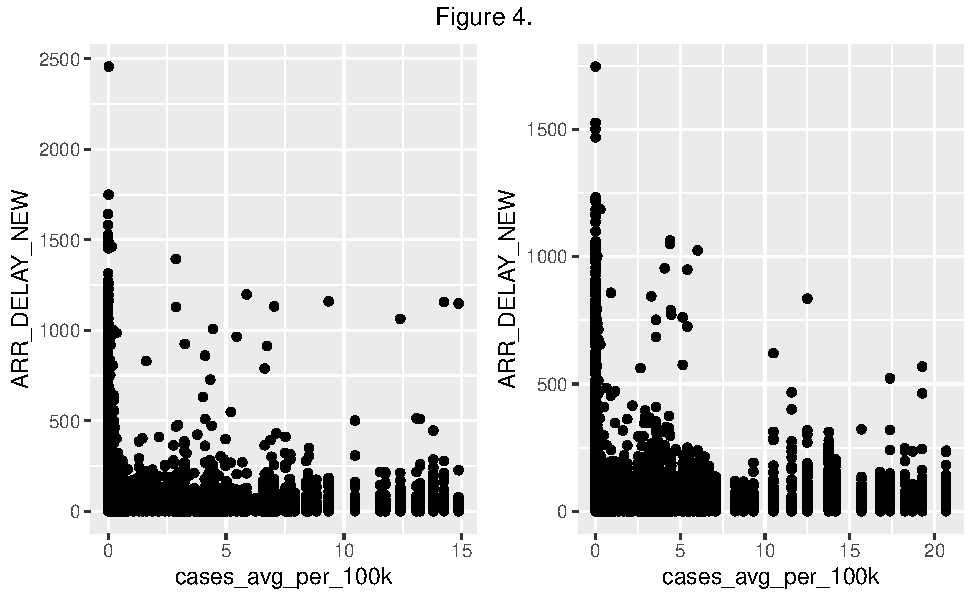
\includegraphics{final-project_files/figure-latex/scatterplot-1.pdf}

\begin{longtable}[]{@{}lr@{}}
\toprule
& 0 \\
\midrule
\endhead
0 & 46658 \\
1 & 4448 \\
\bottomrule
\end{longtable}

\begin{verbatim}
## [1] 0.9129652
\end{verbatim}

\begin{longtable}[]{@{}lr@{}}
\toprule
& 0 \\
\midrule
\endhead
0 & 45517 \\
1 & 5739 \\
\bottomrule
\end{longtable}

\begin{verbatim}
## [1] 0.8880326
\end{verbatim}

\begin{longtable}[]{@{}lrr@{}}
\toprule
& 0 & 1 \\
\midrule
\endhead
0 & 49954 & 1233 \\
1 & 4610 & 1192 \\
\bottomrule
\end{longtable}

\begin{verbatim}
## [1] 0.8974714
\end{verbatim}

\begin{longtable}[]{@{}lrr@{}}
\toprule
& 0 & 1 \\
\midrule
\endhead
0 & 49881 & 1449 \\
1 & 5019 & 1190 \\
\bottomrule
\end{longtable}

\begin{verbatim}
## [1] 0.8875893
\end{verbatim}

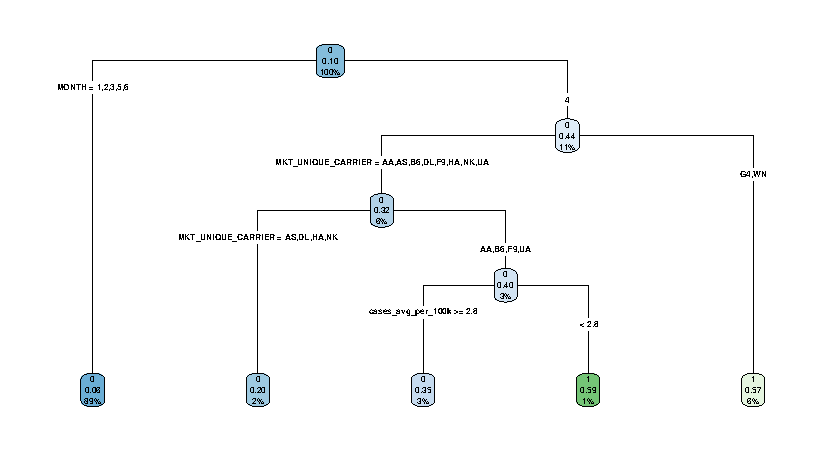
\includegraphics{final-project_files/figure-latex/cancellation-tree-1.pdf}
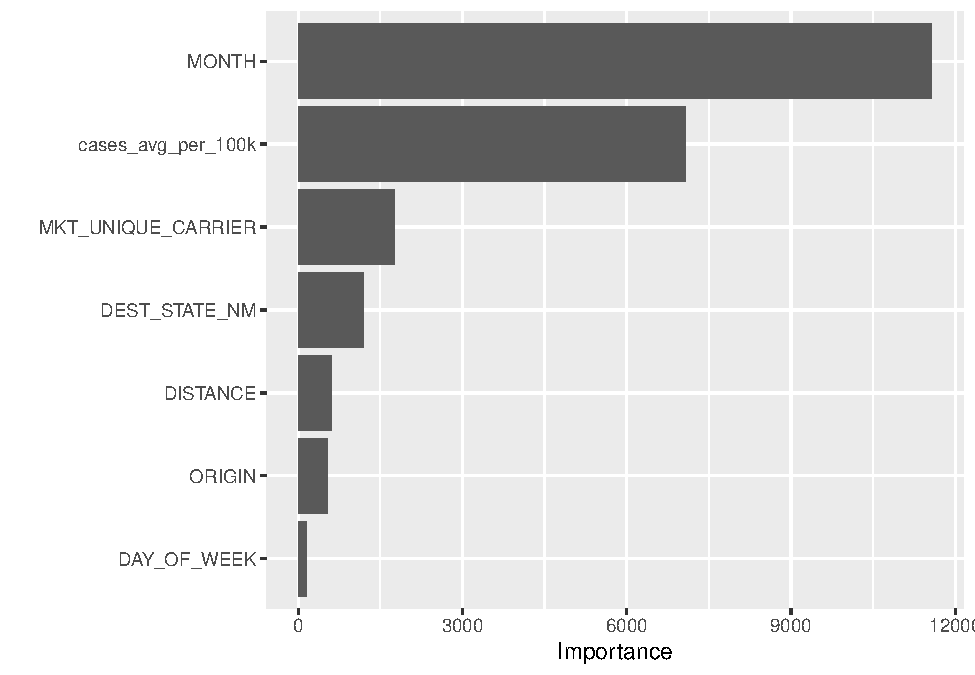
\includegraphics{final-project_files/figure-latex/cancellation-tree-2.pdf}

\begin{verbatim}
## [1] NaN
\end{verbatim}

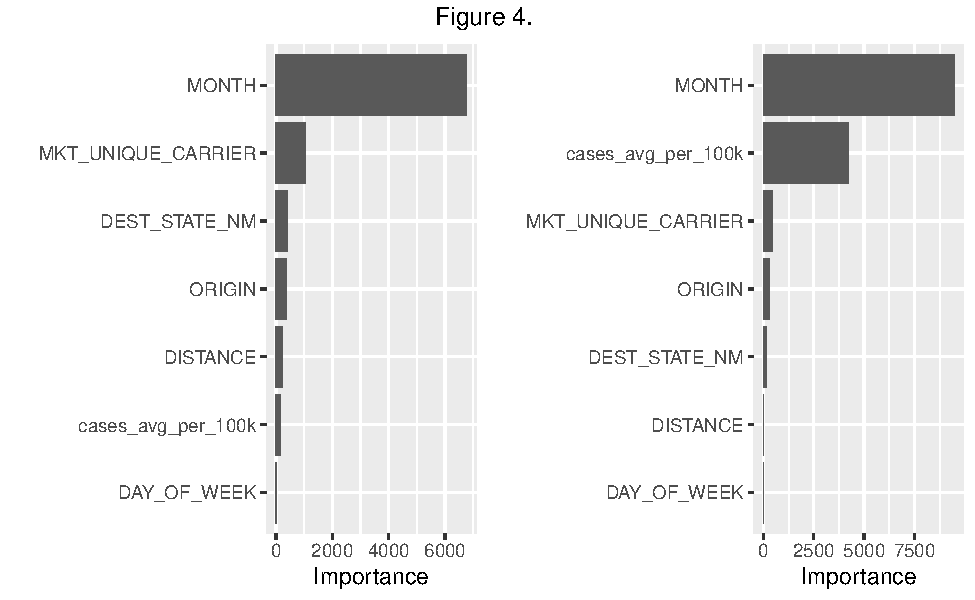
\includegraphics{final-project_files/figure-latex/cancellation-tree-3.pdf}
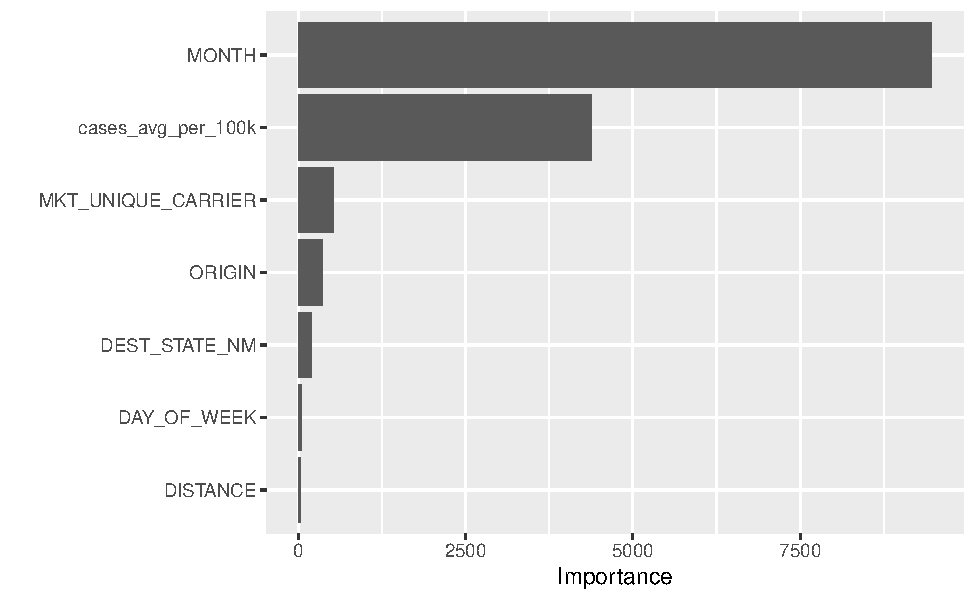
\includegraphics{final-project_files/figure-latex/cancellation-tree-4.pdf}

\begin{verbatim}
## [1] NaN
\end{verbatim}

\begin{verbatim}
## 
## Call:
## lm(formula = ARR_DELAY_NEW ~ MONTH + DAY_OF_WEEK + MKT_UNIQUE_CARRIER + 
##     DISTANCE + cases_avg_per_100k, data = airport_covid_California_train, 
##     na.action = na.omit)
## 
## Residuals:
##     Min      1Q  Median      3Q     Max 
##  -19.85   -8.46   -5.28   -1.74 2448.26 
## 
## Coefficients:
##                        Estimate Std. Error t value Pr(>|t|)    
## (Intercept)          12.0743688  0.3281102  36.800  < 2e-16 ***
## MONTH2               -1.0876161  0.2100580  -5.178 2.25e-07 ***
## MONTH3               -3.0369516  0.2166941 -14.015  < 2e-16 ***
## MONTH4               -6.6555102  0.4343211 -15.324  < 2e-16 ***
## MONTH5               -7.2907144  0.5431907 -13.422  < 2e-16 ***
## MONTH6               -6.7338921  0.8741388  -7.703 1.33e-14 ***
## DAY_OF_WEEK2         -0.6149916  0.2859356  -2.151 0.031493 *  
## DAY_OF_WEEK3         -1.0784439  0.2830749  -3.810 0.000139 ***
## DAY_OF_WEEK4          0.9951280  0.2807329   3.545 0.000393 ***
## DAY_OF_WEEK5          2.3069201  0.2808228   8.215  < 2e-16 ***
## DAY_OF_WEEK6          0.7335559  0.2966442   2.473 0.013405 *  
## DAY_OF_WEEK7          0.9875795  0.2851250   3.464 0.000533 ***
## MKT_UNIQUE_CARRIERAS -2.9390253  0.2903774 -10.121  < 2e-16 ***
## MKT_UNIQUE_CARRIERB6 -2.7271487  0.5056591  -5.393 6.93e-08 ***
## MKT_UNIQUE_CARRIERDL -2.0629765  0.2943464  -7.009 2.41e-12 ***
## MKT_UNIQUE_CARRIERF9 -1.7145425  0.8743083  -1.961 0.049877 *  
## MKT_UNIQUE_CARRIERG4  5.7020463  1.1127428   5.124 2.99e-07 ***
## MKT_UNIQUE_CARRIERHA -2.8714709  0.9511590  -3.019 0.002537 ** 
## MKT_UNIQUE_CARRIERNK -1.8322000  0.6859458  -2.671 0.007562 ** 
## MKT_UNIQUE_CARRIERUA -0.6002482  0.2609938  -2.300 0.021457 *  
## MKT_UNIQUE_CARRIERWN -6.4179120  0.2504224 -25.628  < 2e-16 ***
## DISTANCE             -0.0008816  0.0001116  -7.902 2.75e-15 ***
## cases_avg_per_100k    0.1550709  0.0883141   1.756 0.079107 .  
## ---
## Signif. codes:  0 '***' 0.001 '**' 0.01 '*' 0.05 '.' 0.1 ' ' 1
## 
## Residual standard error: 34.64 on 204144 degrees of freedom
##   (23785 observations deleted due to missingness)
## Multiple R-squared:  0.01101,    Adjusted R-squared:  0.0109 
## F-statistic: 103.3 on 22 and 204144 DF,  p-value: < 2.2e-16
\end{verbatim}

\begin{verbatim}
## [1] 35.59012
\end{verbatim}

\begin{verbatim}
## [1] 30.88132
\end{verbatim}

Beta coefficient = 0.1170830. The partial effect of
cases\_avg\_per\_100k on the airline delay.

\begin{verbatim}
## 
## Call:
## zeroinfl(formula = ARR_DELAY_NEW ~ MONTH + DAY_OF_WEEK + MKT_UNIQUE_CARRIER + 
##     DISTANCE + cases_avg_per_100k | cases_avg_per_100k, data = airport_covid_California_train, 
##     na.action = na.omit)
## 
## Pearson residuals:
##      Min       1Q   Median       3Q      Max 
##  -0.5175  -0.5130  -0.5060  -0.3504 184.9713 
## 
## Count model coefficients (poisson with log link):
##                        Estimate Std. Error  z value Pr(>|z|)    
## (Intercept)           3.846e+00  3.393e-03 1133.464  < 2e-16 ***
## MONTH2                5.598e-03  2.114e-03    2.648 0.008092 ** 
## MONTH3               -2.842e-02  2.365e-03  -12.016  < 2e-16 ***
## MONTH4                5.806e-02  7.332e-03    7.918 2.42e-15 ***
## MONTH5               -5.015e-01  9.376e-03  -53.485  < 2e-16 ***
## MONTH6               -8.763e-01  1.495e-02  -58.631  < 2e-16 ***
## DAY_OF_WEEK2          2.366e-02  3.511e-03    6.737 1.61e-11 ***
## DAY_OF_WEEK3         -1.256e-01  3.532e-03  -35.557  < 2e-16 ***
## DAY_OF_WEEK4         -3.408e-02  3.209e-03  -10.619  < 2e-16 ***
## DAY_OF_WEEK5          7.111e-02  3.093e-03   22.991  < 2e-16 ***
## DAY_OF_WEEK6          1.204e-01  3.399e-03   35.436  < 2e-16 ***
## DAY_OF_WEEK7          7.665e-02  3.254e-03   23.553  < 2e-16 ***
## MKT_UNIQUE_CARRIERAS -3.833e-01  3.035e-03 -126.301  < 2e-16 ***
## MKT_UNIQUE_CARRIERB6 -1.165e-01  5.631e-03  -20.688  < 2e-16 ***
## MKT_UNIQUE_CARRIERDL -1.469e-01  3.005e-03  -48.890  < 2e-16 ***
## MKT_UNIQUE_CARRIERF9 -1.522e-01  8.908e-03  -17.081  < 2e-16 ***
## MKT_UNIQUE_CARRIERG4  1.385e-01  8.389e-03   16.513  < 2e-16 ***
## MKT_UNIQUE_CARRIERHA -4.191e-02  1.152e-02   -3.638 0.000275 ***
## MKT_UNIQUE_CARRIERNK -1.226e-01  7.118e-03  -17.229  < 2e-16 ***
## MKT_UNIQUE_CARRIERUA  9.285e-02  2.491e-03   37.276  < 2e-16 ***
## MKT_UNIQUE_CARRIERWN -7.418e-01  3.025e-03 -245.260  < 2e-16 ***
## DISTANCE             -1.356e-04  8.564e-07 -158.386  < 2e-16 ***
## cases_avg_per_100k    5.048e-02  1.393e-03   36.235  < 2e-16 ***
## 
## Zero-inflation model coefficients (binomial with logit link):
##                    Estimate Std. Error z value Pr(>|z|)    
## (Intercept)        1.296026   0.006114  211.97   <2e-16 ***
## cases_avg_per_100k 0.111545   0.002519   44.28   <2e-16 ***
## ---
## Signif. codes:  0 '***' 0.001 '**' 0.01 '*' 0.05 '.' 0.1 ' ' 1 
## 
## Number of iterations in BFGS optimization: 1 
## Log-likelihood: -1.332e+06 on 25 Df
\end{verbatim}

\begin{verbatim}
## [1] 35.51814
\end{verbatim}

\begin{verbatim}
## 
## Call:
## zeroinfl(formula = ARR_DELAY_NEW ~ MONTH + DAY_OF_WEEK + MKT_UNIQUE_CARRIER + 
##     DISTANCE + cases_avg_per_100k | cases_avg_per_100k, data = airport_covid_Texas_train, 
##     na.action = na.omit)
## 
## Pearson residuals:
##      Min       1Q   Median       3Q      Max 
##  -0.5637  -0.5590  -0.5514  -0.4566 117.7892 
## 
## Count model coefficients (poisson with log link):
##                        Estimate Std. Error  z value Pr(>|z|)    
## (Intercept)           3.657e+00  2.727e-03 1340.716  < 2e-16 ***
## MONTH2               -1.320e-01  2.073e-03  -63.703  < 2e-16 ***
## MONTH3               -7.932e-02  2.214e-03  -35.831  < 2e-16 ***
## MONTH4               -3.431e-01  4.773e-03  -71.881  < 2e-16 ***
## MONTH5               -3.762e-01  4.486e-03  -83.867  < 2e-16 ***
## MONTH6               -5.321e-01  7.175e-03  -74.161  < 2e-16 ***
## DAY_OF_WEEK2         -1.666e-01  3.248e-03  -51.290  < 2e-16 ***
## DAY_OF_WEEK3         -1.169e-01  3.089e-03  -37.839  < 2e-16 ***
## DAY_OF_WEEK4         -1.998e-02  2.850e-03   -7.012 2.36e-12 ***
## DAY_OF_WEEK5          4.488e-02  2.809e-03   15.979  < 2e-16 ***
## DAY_OF_WEEK6          1.171e-02  3.130e-03    3.742 0.000182 ***
## DAY_OF_WEEK7         -3.954e-02  3.023e-03  -13.077  < 2e-16 ***
## MKT_UNIQUE_CARRIERAS -1.931e-01  7.783e-03  -24.812  < 2e-16 ***
## MKT_UNIQUE_CARRIERB6  2.186e-01  1.162e-02   18.813  < 2e-16 ***
## MKT_UNIQUE_CARRIERDL  1.710e-01  3.682e-03   46.441  < 2e-16 ***
## MKT_UNIQUE_CARRIERF9  3.831e-01  9.809e-03   39.054  < 2e-16 ***
## MKT_UNIQUE_CARRIERG4  3.118e-01  1.111e-02   28.064  < 2e-16 ***
## MKT_UNIQUE_CARRIERNK  1.004e-01  5.711e-03   17.581  < 2e-16 ***
## MKT_UNIQUE_CARRIERUA  7.508e-02  1.987e-03   37.790  < 2e-16 ***
## MKT_UNIQUE_CARRIERWN -4.269e-01  2.605e-03 -163.918  < 2e-16 ***
## DISTANCE             -3.763e-05  1.416e-06  -26.582  < 2e-16 ***
## cases_avg_per_100k    2.035e-02  5.590e-04   36.408  < 2e-16 ***
## 
## Zero-inflation model coefficients (binomial with logit link):
##                    Estimate Std. Error z value Pr(>|z|)    
## (Intercept)        1.123907   0.005714  196.68   <2e-16 ***
## cases_avg_per_100k 0.028292   0.001567   18.05   <2e-16 ***
## ---
## Signif. codes:  0 '***' 0.001 '**' 0.01 '*' 0.05 '.' 0.1 ' ' 1 
## 
## Number of iterations in BFGS optimization: 1 
## Log-likelihood: -1.473e+06 on 24 Df
\end{verbatim}

\begin{verbatim}
## [1] 30.88815
\end{verbatim}

For the zero-inflated poisson model, the first process generates zeros
and the second process is governed by a Poisson distribution that
generates counts, some of which may be zero. In this model building, the
assumption is that the covid cases would generate the non-zero counts.

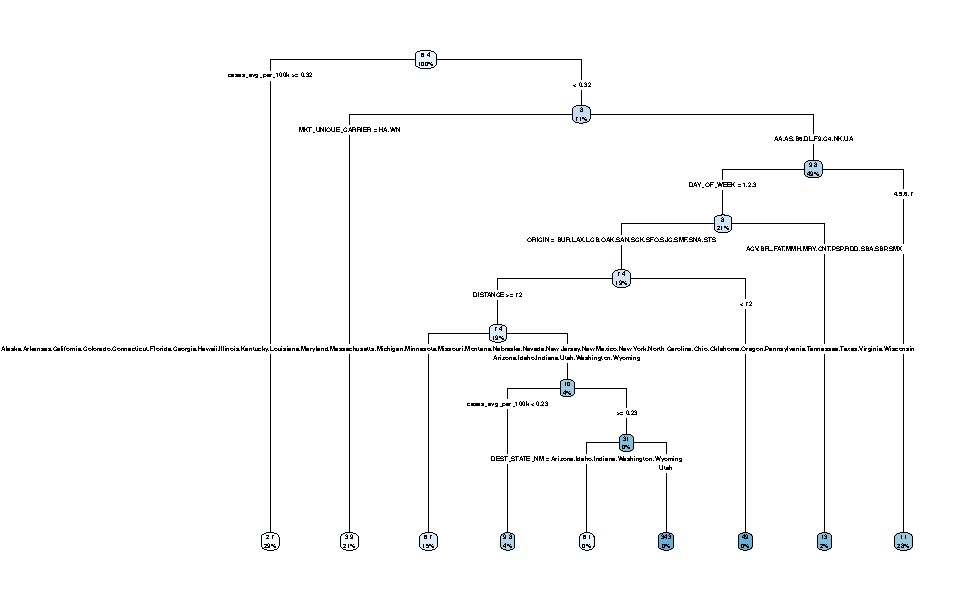
\includegraphics{final-project_files/figure-latex/delay-tree-1.pdf}
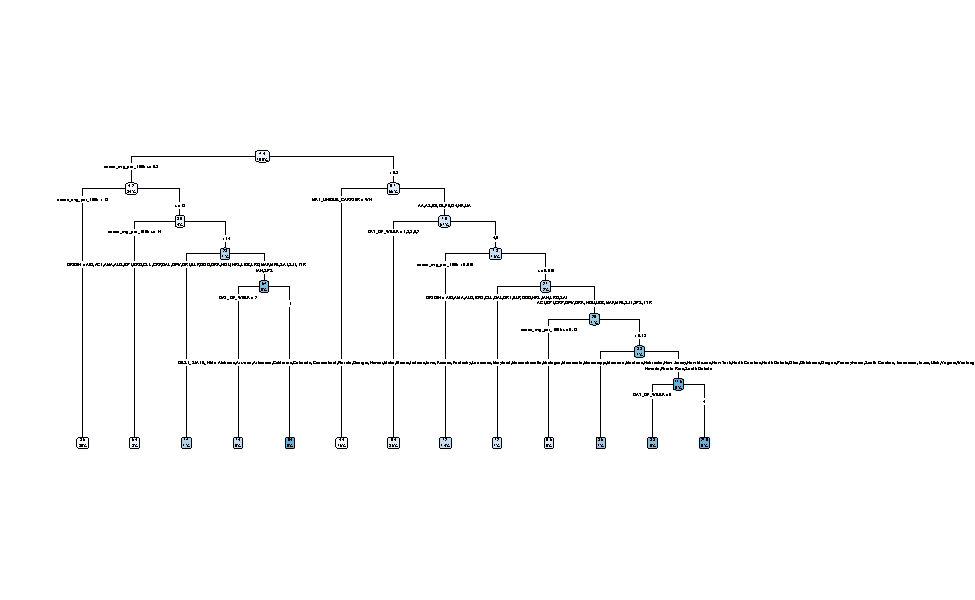
\includegraphics{final-project_files/figure-latex/delay-tree-2.pdf}

\begin{verbatim}
## [1] 35.22869
\end{verbatim}

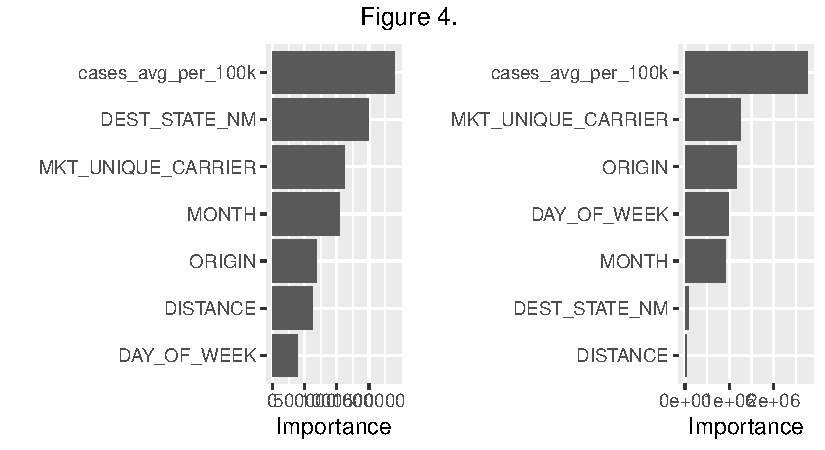
\includegraphics{final-project_files/figure-latex/delay-tree-3.pdf}
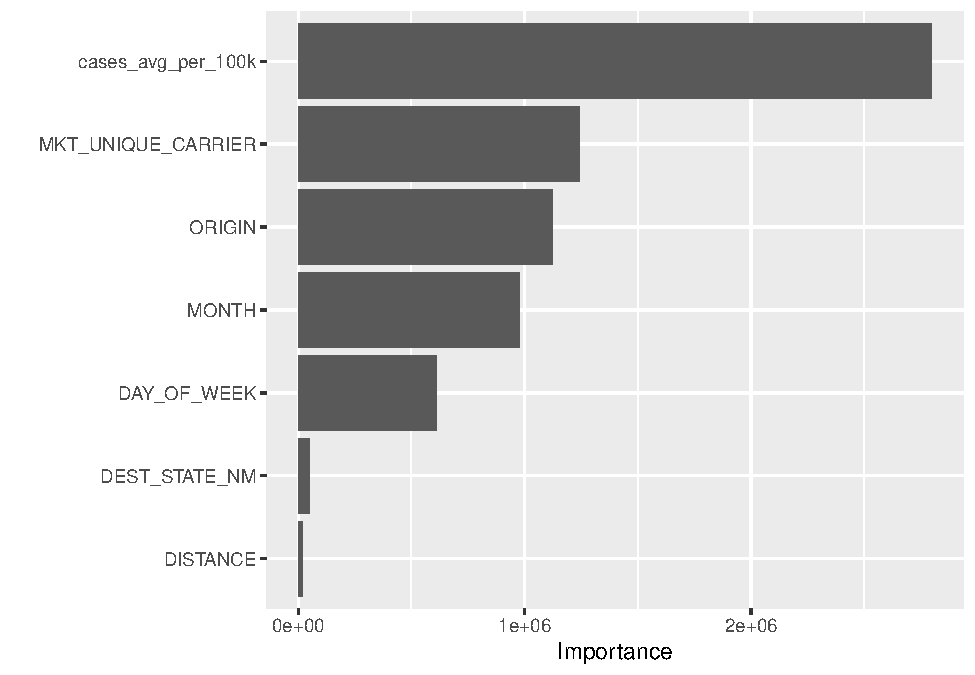
\includegraphics{final-project_files/figure-latex/delay-tree-4.pdf}

\begin{verbatim}
## [1] 30.32028
\end{verbatim}

\begin{verbatim}
## [1] 98.84347
\end{verbatim}

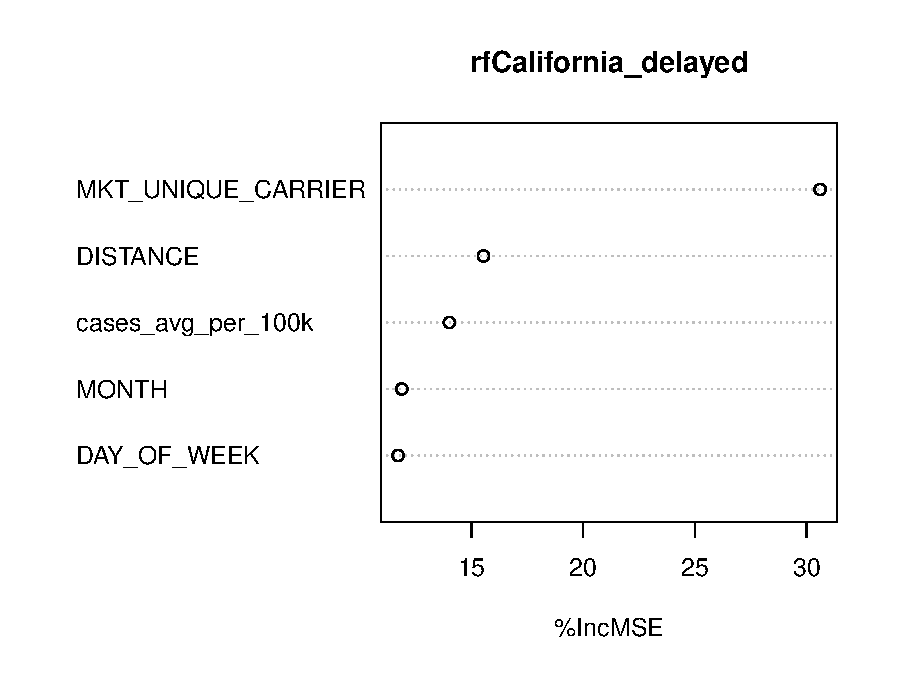
\includegraphics{final-project_files/figure-latex/rf-delaytime-1.pdf}
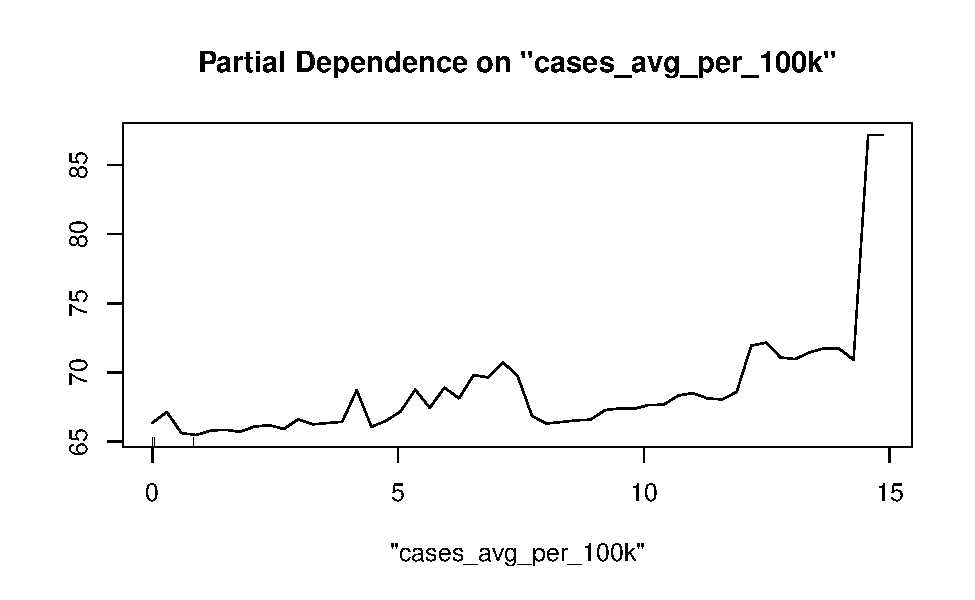
\includegraphics{final-project_files/figure-latex/rf-delaytime-2.pdf}

\begin{verbatim}
## [1] 82.96199
\end{verbatim}

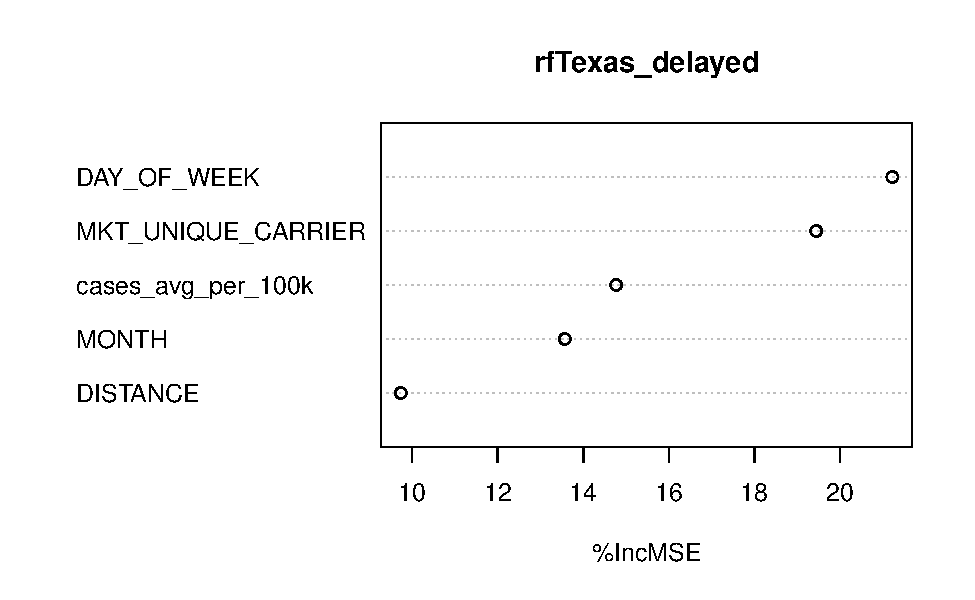
\includegraphics{final-project_files/figure-latex/rf-delaytime-3.pdf}
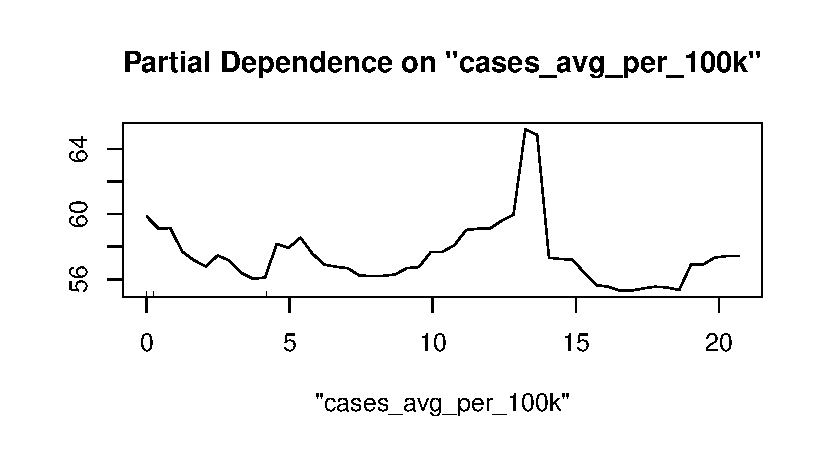
\includegraphics{final-project_files/figure-latex/rf-delaytime-4.pdf}

Including \texttt{ORIGIN} only reduced the rMSE from 97.35954 to
97.20708. removing the variable for the entire country analysis, as
there are too many levels.

\end{document}
